\chapter{Event Reconstruction}
\label{ch:evtReco}

\begin{chapquote}{Hebrews 11:3}
{The things which are seen are not made of the things which do appear.}
\end{chapquote}

The task of event reconstruction involves taking electronic read out signals from the 100 million sensors in the detector and to reconstruct objects that can serve as proxies to the physics observables (i.e, $b$-quarks) % from a HIggs decay)
that to use in high-level physics analysis.
Since the LHC collides protons, %, three quarks held together by gluons
we produce lots of quarks and gluons in the final state, with an example of the signature these particles produce in the detector shown in \Fig{\ref{fig:tracks-clusters-annotated}}.

\begin{figure}[hbt]
\centering
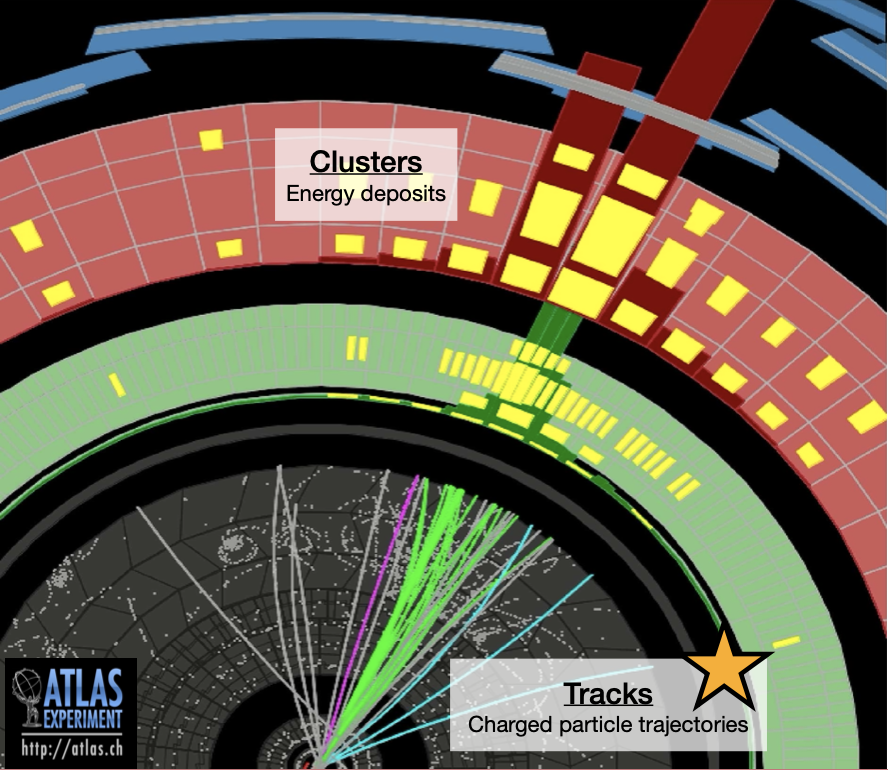
\includegraphics[width=.6\textwidth]{figures/cp-graphics/tracks-clusters-annotated}
\caption{Illustration of what a jet looks like in our detector}
\label{fig:tracks-clusters-annotated}
\end{figure}

Since this thesis deals with an analysis with an all-hadronic final states, these are the key input objects for the analysis and for my work in \Pqb-tagging, so in this chapter we focus on the reconstruction of these types of events.
We include this graphic here, because it nicely demonstrates the outline for this chapter
The charged particle trajectories in the inner detector form a set of tracks, and will be described in \Sect{\ref{sec:tracks}}.
The tracks that originate from the same location are then reconstructed into vertices, as described in \Sect{\ref{sec:vertices}}.
The unsupervised learning algorithms that get reconstructs the quark and gluon decay products into the ``jets'' are described in \Sect{\ref{sec:jets}}.
Finally, we conclude with the reconstruction muon tracks in \Sect{\ref{sec:muons}}.


\textbf{Citation:} The European Physical Journal C Vol 73 3 (2013) 2304
% Note - if I include this, I \emph{know} that Pat will ask me about the details, so I should make sure I understand the color coding, etc.

\section{Tracks}
\label{sec:tracks}

\subsection{Track reconstruction}

To cite: \cite{soft-pub-2007-007}

\textbf{Inside out:}
\begin{itemize}
	\item Cluster formation
	\item Seed finding: reco triplets of hits from the pixel detector
	\item Track fitting with a combinatorial Kalman filter
	\item Ambiguity solving of which hits with a collection of NNs which decides whether a given cluster is shared between two tracks and how to split the energy depostion between these multiple tracks \cite{jinst-9-2014-P09009}
	\item Extend to the TRT hits
\end{itemize}

Improve the efficiency due to tracks in that have decays displaced from the original collision point with an \textbf{outside in:} track reconstruction alrogihm
\begin{itemize}
	\item Start with the seeds from the TRT
	\item Extend to the hits in the silicon detector
	\item Again use an ambiguity solver.
\end{itemize}

\begin{figure}[hbt]
\centering
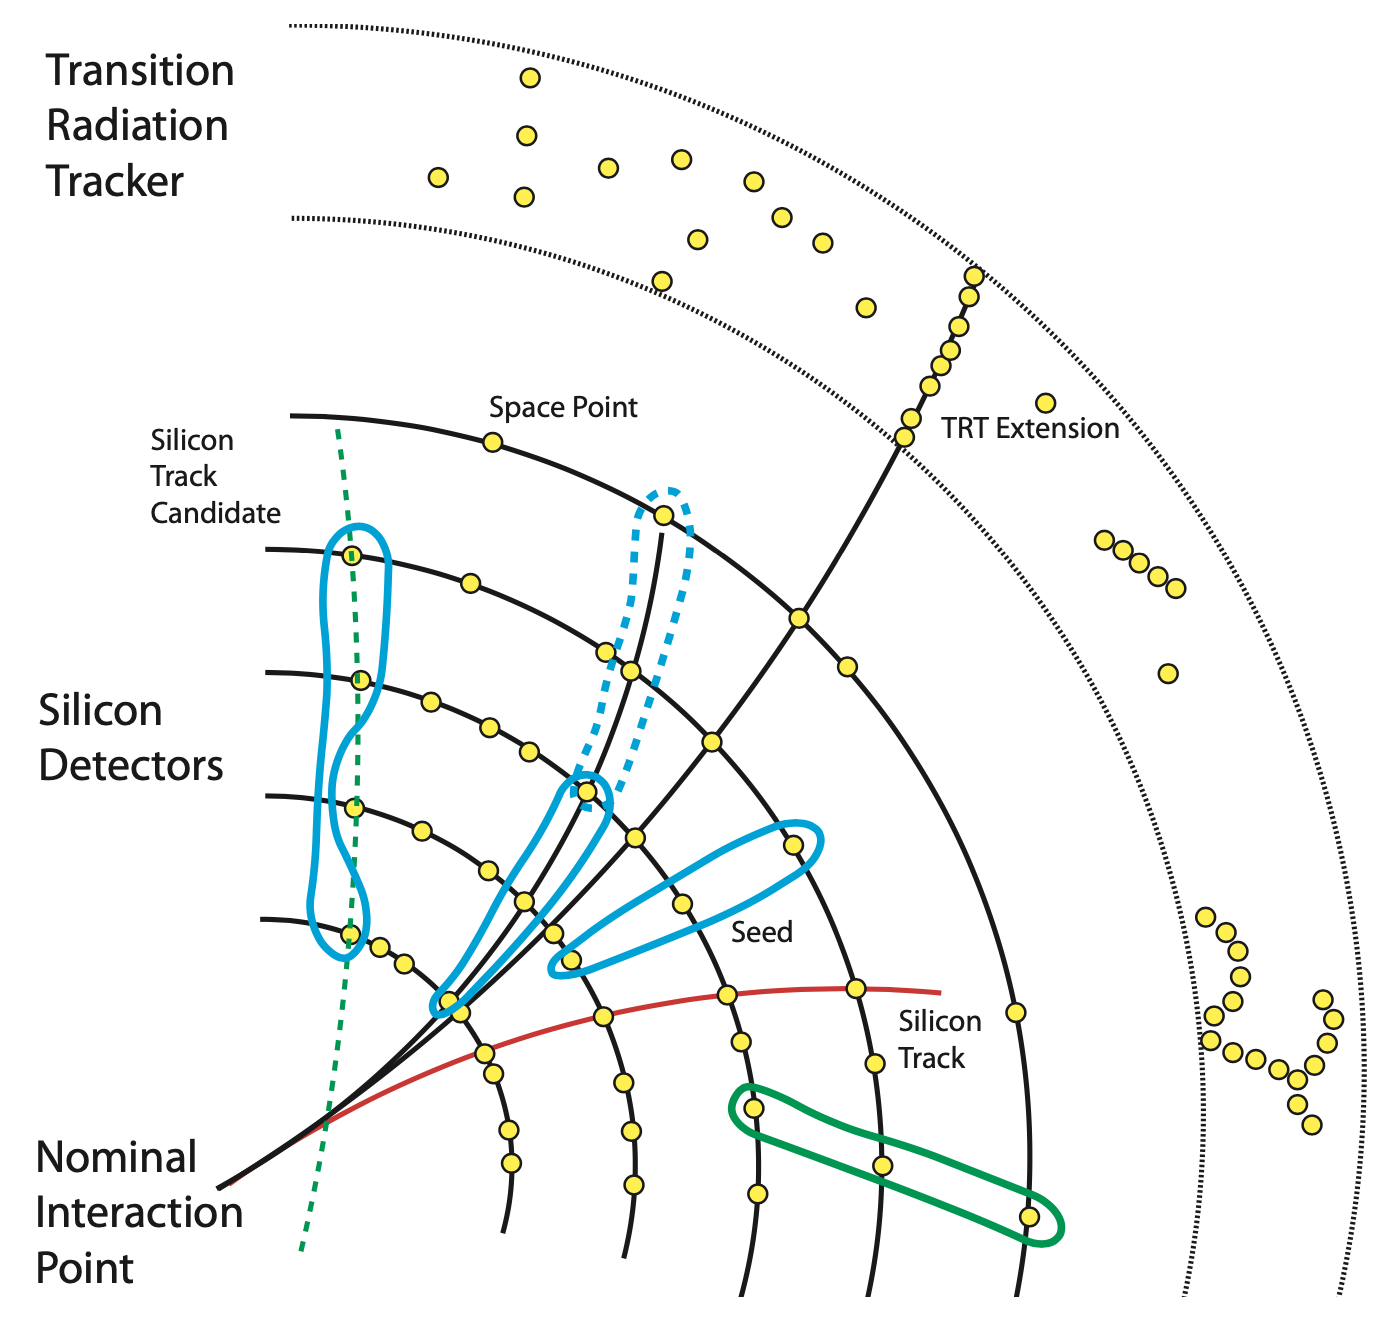
\includegraphics[width=0.6\textwidth]{figures/cp-graphics/tracking/track-reco}
\caption{\hl{need to ask Valentina where this pic was from originally}.}
\label{fig:track-reco}
\end{figure}


\subsection{Challenges in Dense Environments}

\begin{figure}[hbt]
\centering
\subfloat[]{
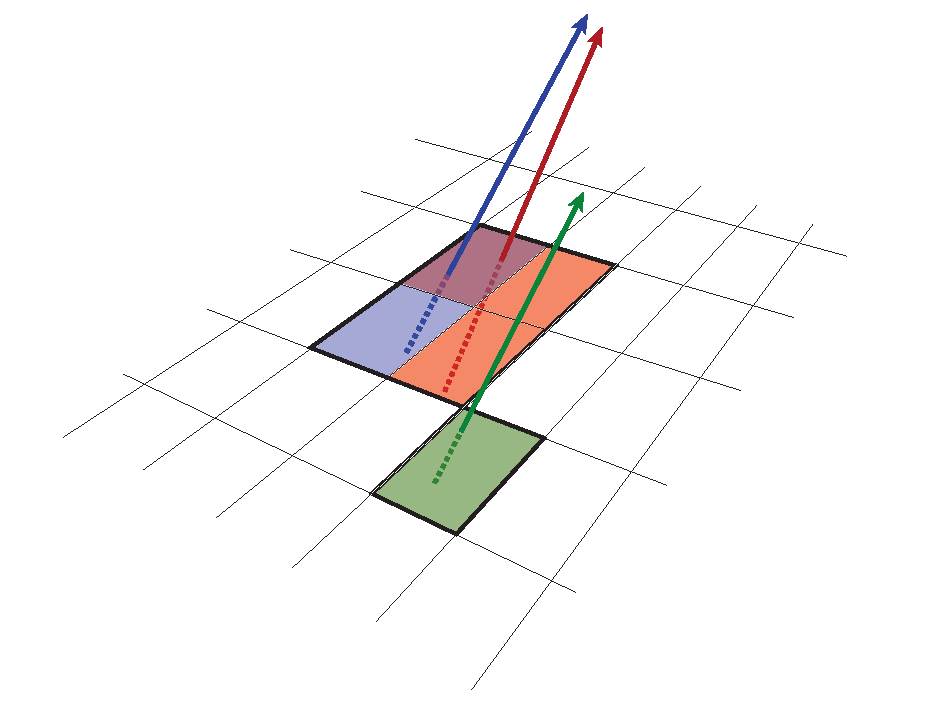
\includegraphics[width=0.43\textwidth]{figures/cp-graphics/jinst-9-2014-P09009/fig_03}
}
\subfloat[]{
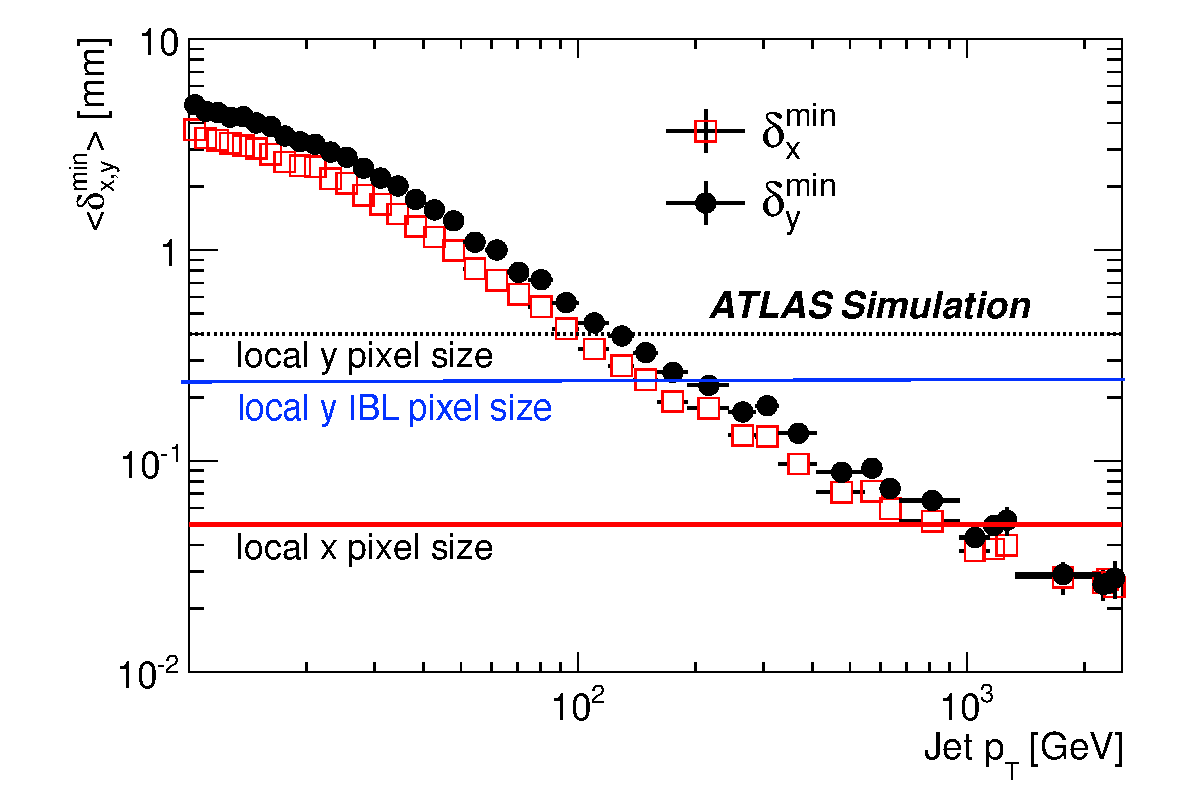
\includegraphics[width=0.55\textwidth]{figures/cp-graphics/jinst-9-2014-P09009/fig_04}
}
\caption{\cite{jinst-9-2014-P09009}.}
\label{fig:ctide}
\end{figure}


\subsection{Discussion of inputs}


\begin{figure}[hbt]
\centering
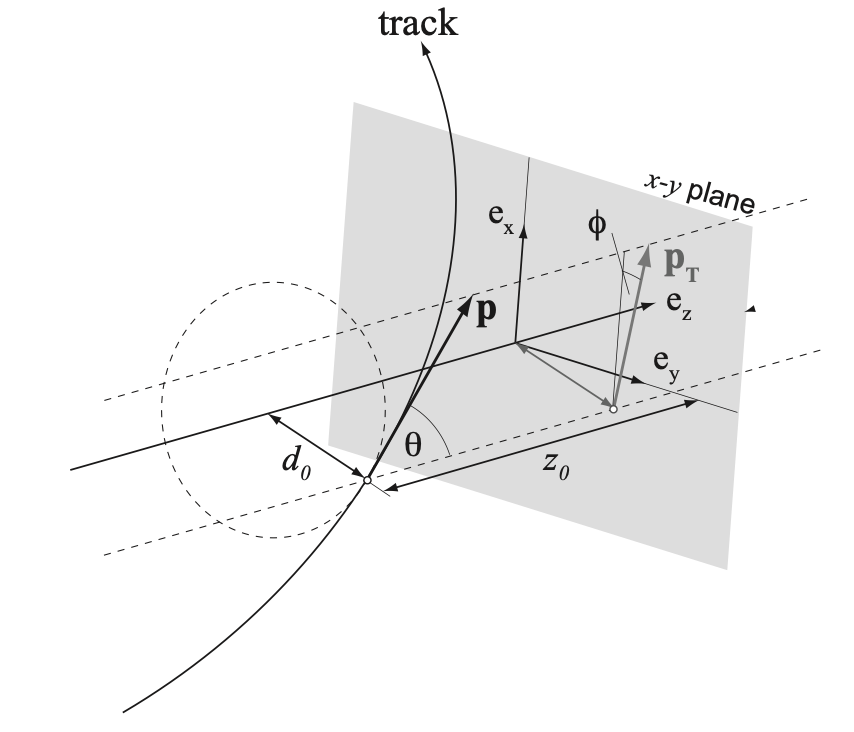
\includegraphics[width=0.6\textwidth]{figures/cp-graphics/ATL-SOFT-PUB-2007-003/fig-2a}
\caption{\cite{ATL-SOFT-PUB-2007-003}}
\label{fig:ATL-SOFT-PUB-2007-003-fig-2a}
\end{figure}

\begin{figure}[hbt]
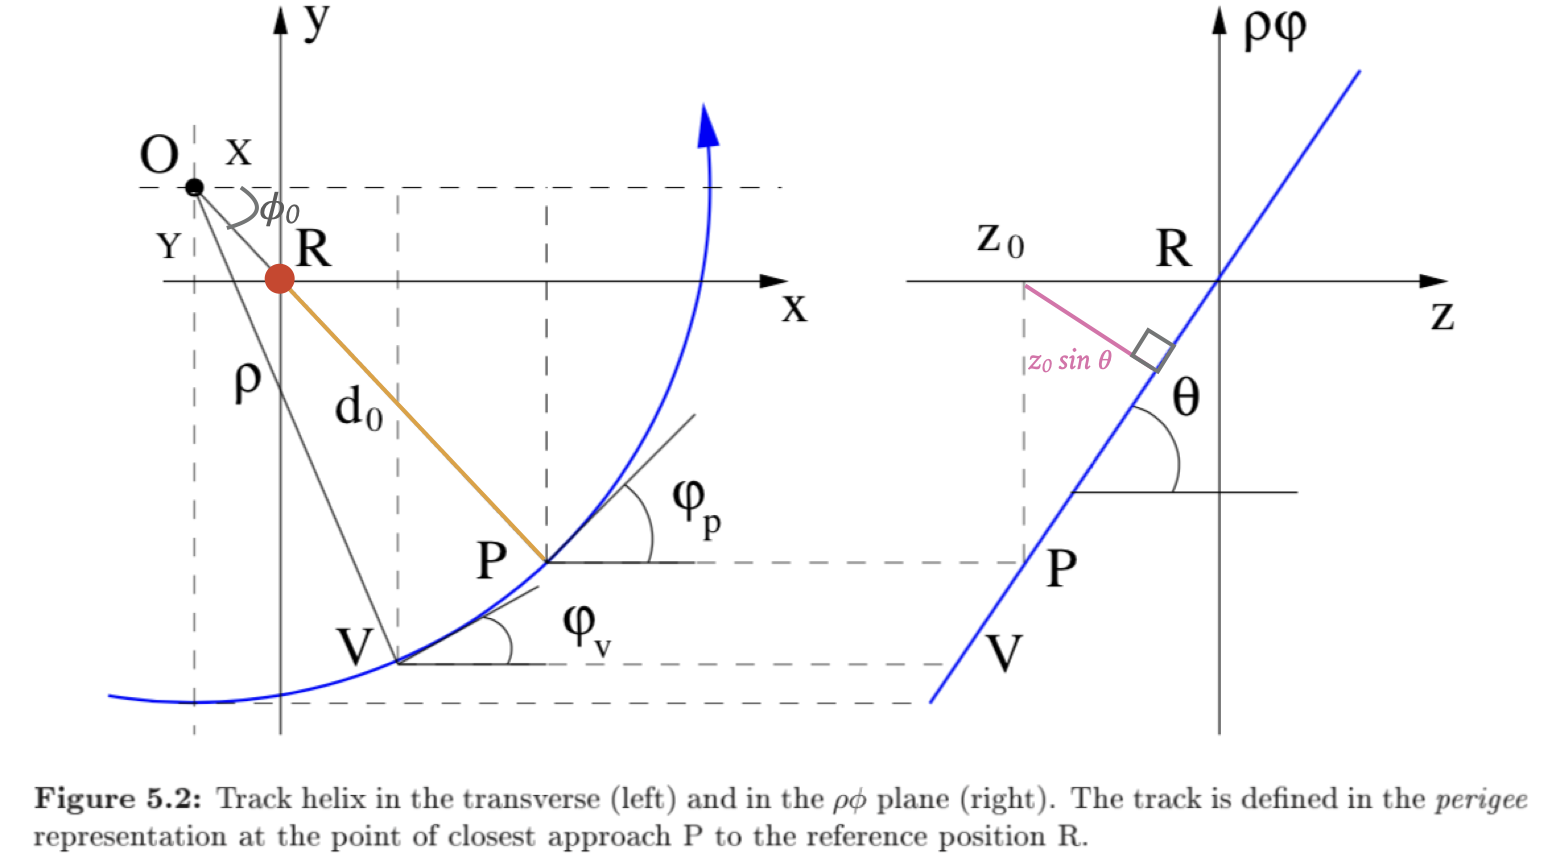
\includegraphics[width=\textwidth]{figures/cp-graphics/giacinto-fig-5.2}
\caption{\cite{giacinto-thesis}}
\label{fig:track-2d-graphics}
\end{figure}

\begin{itemize}
	\item \textcolor{red}{R}: reference position at which the tracks are defined, i.e, for \Pqb-tagging we use the primary vertex of the collision as the reference point. 
	\item \textcolor{orange}{$d_0$}:  The transverse impact parameter, point of closest approach (POCA) in the transverse plane with respect to R.
	\item \textcolor{pink}{$z_0 \sin \theta$}:  The longitudinal impact parameter, or the longitudinal displacement from the POCA (defined in the transverse plane). The multiplication by $\sin \theta$ term is included because it characterizes the 2d distance from $z_0$ to the closest point along the track trajectory.
\end{itemize}


\begin{align}
x_V &= x_R + d_0 \cos \left( \phi_p + \frac{\pi}{2} \right)+ \rho \left[  \cos \left( \phi_V + \frac{\pi}{2}  -  \cos \left( \phi_p + \frac{\pi}{2} \right)\right)  \right] \notag \\
y_V &= y_R + d_0 \sin \left( \phi_p + \frac{\pi}{2} \right)+ \rho \left[  \sin \left( \phi_V + \frac{\pi}{2}  -  \sin \left( \phi_p + \frac{\pi}{2} \right)\right)  \right] \\
z_V &= z_R + z_0 - \frac{\rho}{\tan \left( \theta \right) } \left[ \phi_V - \phi_p \right] \notag
\end{align}

\begin{figure}[hbt]
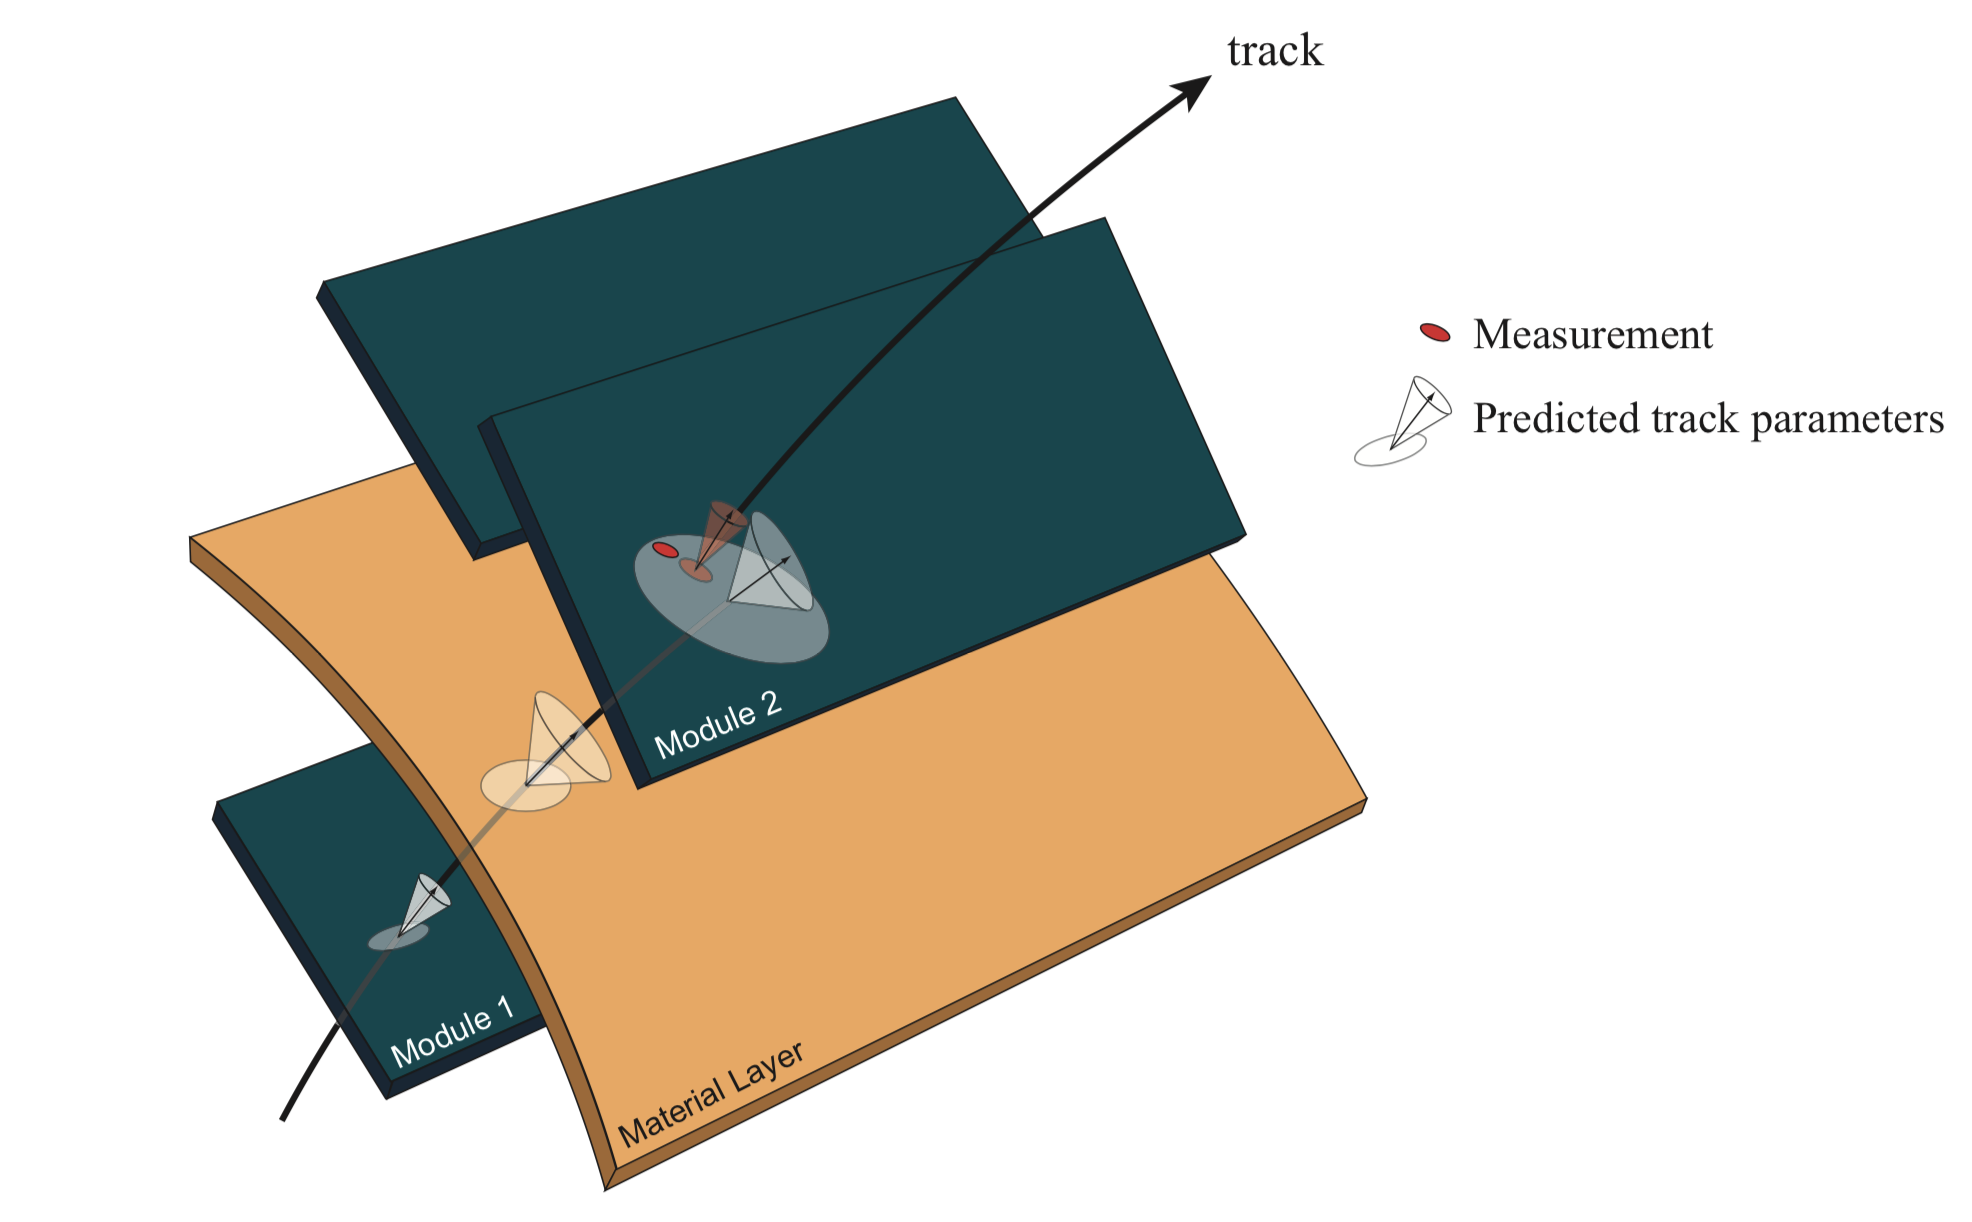
\includegraphics[width=\textwidth]{figures/cp-graphics/ATL-SOFT-PUB-2007-005/track-extrap-material-int}
\caption{Visualization of the track extrapolation with its associated errors \cite{ATL-SOFT-PUB-2007-005}.}
\label{fig:track-extrap-material-int}
\end{figure}

\begin{equation}
\rho = \frac{\sin \theta}{\frac{q}{p} B_z}
\end{equation}

\begin{align}
d_0 &= \text{sign} \left( d_0 - \rho \right) \sqrt{\left(x_V - x_R - \rho \cos \left(\phi_V + \frac{\pi}{2} \right) \right)^2 +  \left(y_V - y_R - \rho \sin \left(\phi_V + \frac{\pi}{2} \right) \right)^2 } \\
\phi_p &= \arctan \left( \frac{y_V - y_R - \rho \sin \left( \phi_V + \frac{\pi}{2}\right)}{x_V - x_R - \rho \cos \left( \phi_V + \frac{\pi}{2}\right)} \right) \\
z_0 &= z_R + z_V + \frac{\rho}{\tan \theta } \left[ \phi_V - \phi_p (x_V, y_V, z_V, \theta, q/p) \right]\\
\left( \frac{q}{p} \right)_P &= \left( \frac{q}{p} \right)_V \\
\theta_P &= \theta_V
\end{align}

The way we map from one representation to another is by calculating the Jacobians of the transformations:

\begin{equation}
A = \frac{\partial (d_0, z_0, \phi_P, \theta_P, q/p)}{\partial (x_V, y_V, z_V)} = 
\begin{bmatrix}
- h \frac{X}{S} & - h \frac{Y}{S} & 0 \\
\frac{\rho}{\tan \theta}  \frac{Y}{S^2} & - \frac{\rho}{\tan \theta}  \frac{X}{S^2}  & 1 \\
- \frac{Y}{S^2} &  \frac{X}{S^2} & 0 \\
0 & 0 & 0 \\
0 & 0 & 0
\end{bmatrix}
\end{equation}

\begin{equation}
B =  \frac{\partial (d_0, z_0, \phi_P, \theta_P, q/p)}{\partial (\phi_V, \theta, q/p)} = 
\begin{bmatrix}
- \frac{h \rho}{S} R & \frac{\rho}{\tan \theta} \left[ 1 - \frac{h}{S} R \right]  & - \frac{\rho}{q/p} \left[ \Delta \phi - \frac{h}{S} R  \right]  \\
\frac{\rho}{\tan \theta}  \left[ 1 - \frac{\rho}{S^2} Q \right] & \rho \left[ \Delta \phi + \frac{\rho}{S^2 \tan^2 \theta } R \right] & \frac{\rho}{q/p \tan \theta}\left[ \Delta \phi - \frac{\rho}{S^2} R \right] \\
\frac{\rho}{S^2} Q & - \frac{\rho}{S^2 \tan \theta}   R & \frac{\rho}{S^2 q/p}   R \\
0 & 1 & 0 \\
0 & 0 & 1 
\end{bmatrix}
\end{equation}


where:
\begin{align*}
X &= x_V - x_R - \rho \cos \left(\phi_V + \frac{\pi}{2} \right) 
Y &= y_V - y_R - \rho \sin \left( \phi_V + \frac{\pi}{2}\right)
R &= Y \sin \phi_V + X \cos \phi_V \\
Q &= X \sin \phi_V - Y \cos \phi_V \\
S &= \sqrt{X^2 + Y^2} \\
h &= \text{sign}  \rho \\
\phi &= \phi_P - \phi_V
\end{align*}

\textbf{Q:} How do we define the sign of $\rho$?

\subsection{The perigee parameters}

\FloatBarrier
\clearpage
\section{Vertexing}
\label{sec:vertexing}

\subsection{General problem formulation}

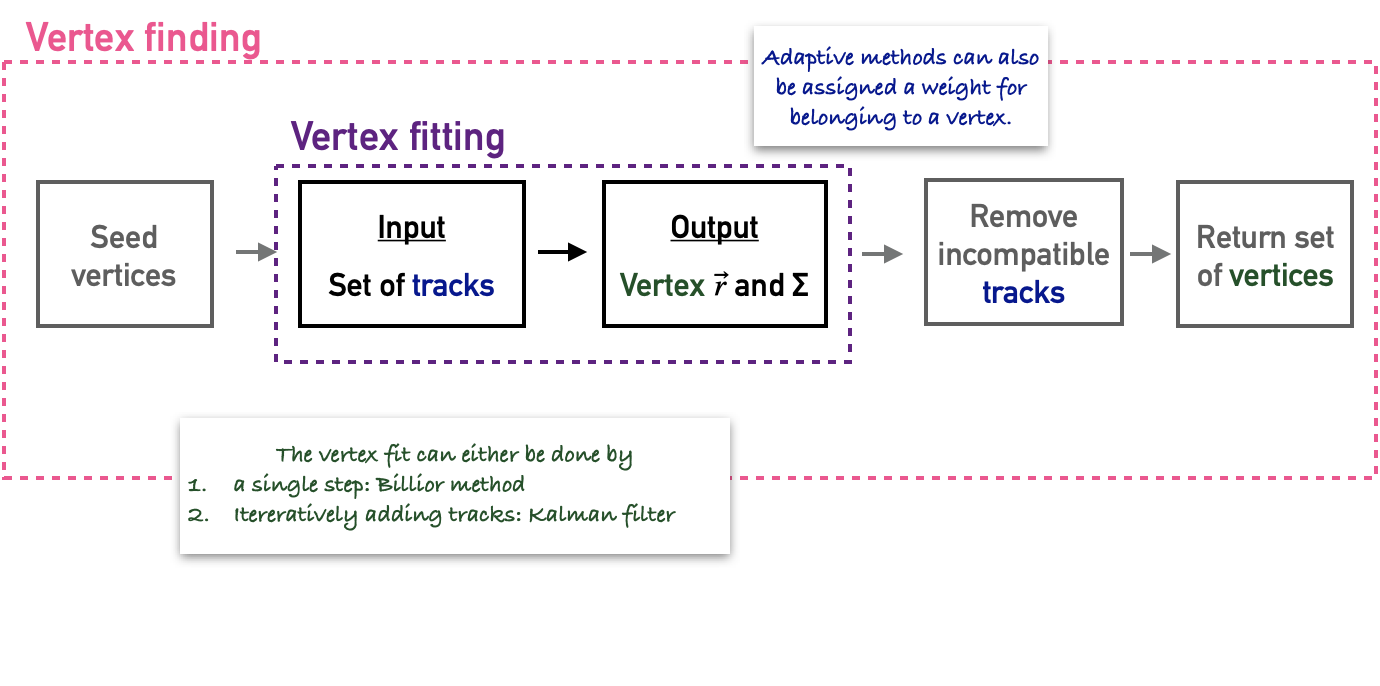
\includegraphics[width=\textwidth]{figures/cp-graphics/Vertex-finding-fitting}

The \textcolor{rebeccapurple}{Vertex fit:} Position which maximizes the likelihood for the probability density tubes for the tracks to all intersect at this point \cite{giacinto-thesis}. 
This is seen mathematically by \Eq{\ref{eq:vtx-prob-density-fct}} below, where $\vec{r}$ is the position of the vertex, and $\vec{r}_i(\phi_{p,i})$ is track $i$ and $\phi_{p,i}$ parametrizes what point of the trajectory that we're on.

\begin{equation}
P(\vec{r}) = \int d \phi_{p,1} d \phi_{p,2} \ldots d \phi_{p,n} \prod_{i=1}^{n_{trk}} 
\exp \left[ - \frac{1}{2}  \left(\vec{r} - \vec{r}_i (\phi_{i,i})\right)^T COV^{-1}_{3x3} (\phi_{p,i}) \left(\vec{r} - \vec{r}_i (\phi_{i,i})\right) \right]
\label{eq:vtx-prob-density-fct}
\end{equation}

\hl{Is this cov matrix the vertex cov? If so, should I call it $\Sigma$ instead of $Cov_{3x3}$?}

\subsection{Primary vertex reconstruction}

The event's selected primary vertex (PV) is defined as the reconstructed primary vertex with largest $\sum \pT^2$ of the associated tracks. 


\clearpage
\section{Jets}

\subsection{Jet clustering algorithms}

A given $pp$ collision produces many quarks and gluons.  However, because of the ``confinement principle,'' no free color charge can exist, which means no isolated quarks or gluons can exist in nature. %\cite{SM_Higgs, Particle_World}.  
It becomes energetically favorable for quark / anti-quark pairs to pop out of the vacuum to balance the color charge imbalance by forming color neutral hadrons. 
This sparks a chain reaction which produces a spray of particles in the detector. 

The anti-k$_T$ algorithm provides a way to cluster the energy deposited in the calorimeter to form a ``jet,'' and is the standard algorithm for defining jets at ATLAS \cite{antiKt}.  First it defines two quantities, 
%
\begin{equation}
d_{ij} = {\text{min}}( p_{Ti}^{-2}, p_{Tj}^{-2}) \frac{\Delta R_{ij}}{R^2} \qquad \qquad  d_i = p_{Ti}^{-2}
\end{equation}
%
where $\Delta R_{ij}^2 = (y_i - y_j)^2 + (\phi_i - \phi_j)^2$, and $R$ is the jet-radius, defined by the user.  To find the jets, the algorithm
%
\begin{itemize}
\item{Calculates $d_{ij}$ and $d_i$ for all particles in the event, and lets $d$ be the smallest $d_i$, $d_{ij}$.}
%\item{Find all the $d_{ij}$ and $d_i$ in the event, and let $d = min(\{d_{ij}, D_i\})$}
	\begin{itemize}
	\item{If $d = d_{ij}$, then it combines jet $i$ and jet $j$.}
	\item{If $d = d_{i}$, then it lets jet $i$ be the final jet.}
	\end{itemize}
\item{It continues the previous steps until all the particles in the event have been accounted for.}
\end{itemize}
%
This algorithm clusters high-$p_T$ particles together if they fall within the jet's radius. \\

The $pp$ collisions at 13~TeV typically will give rise to about 20 moderate $p_T$ jets in the detector, or around ${{20}\choose{2}} = 190$ viable di-jet candates.  So the challenge in elucidating the $H\rightarrow b\bar{b}$ or $HH \rightarrow 4b$ signals is accurately finding the ``correct'' pair(s) of jets.

Since the protons are not point-like, the colliding partons may not have equal $p_T$ in the lab frame. By definition, the net momentum will be zero in the center of mass (CM) frame.  A heavy ($\sim$TeV) resonance can be created at (or nearly at) rest in the CM frame, but when Lorentz boosting back into the lab frame the decay products can become highly collimated.  When the decay products can no longer be resolved individually, we instead search for jets with a large radius parameter (``fat jets''), indicative of merged jets \cite{SM_Higgs, Merged_Jets}.  The constituent clusters inside a fat jet are called \emph{subjets}.  
Large R (about 1.0) correspond to fat jets, and R about 0.4 correspond to the standard resolved jets.

\subsection{PFlow}

\emph{Why better?}

\textbf{To cite for pT plot:}
2007.02645 \\
Eur. Phys. J. C 81 (2021) 689

\textbf{To cite for $\phi$ plot:}
https://indico.cern.ch/event/777980/contributions/3236356/subcontributions/271401/attachments/1780062/2896765/JESJER.pdf

\begin{figure}
\centering
\subfloat[\pt resolution]{
	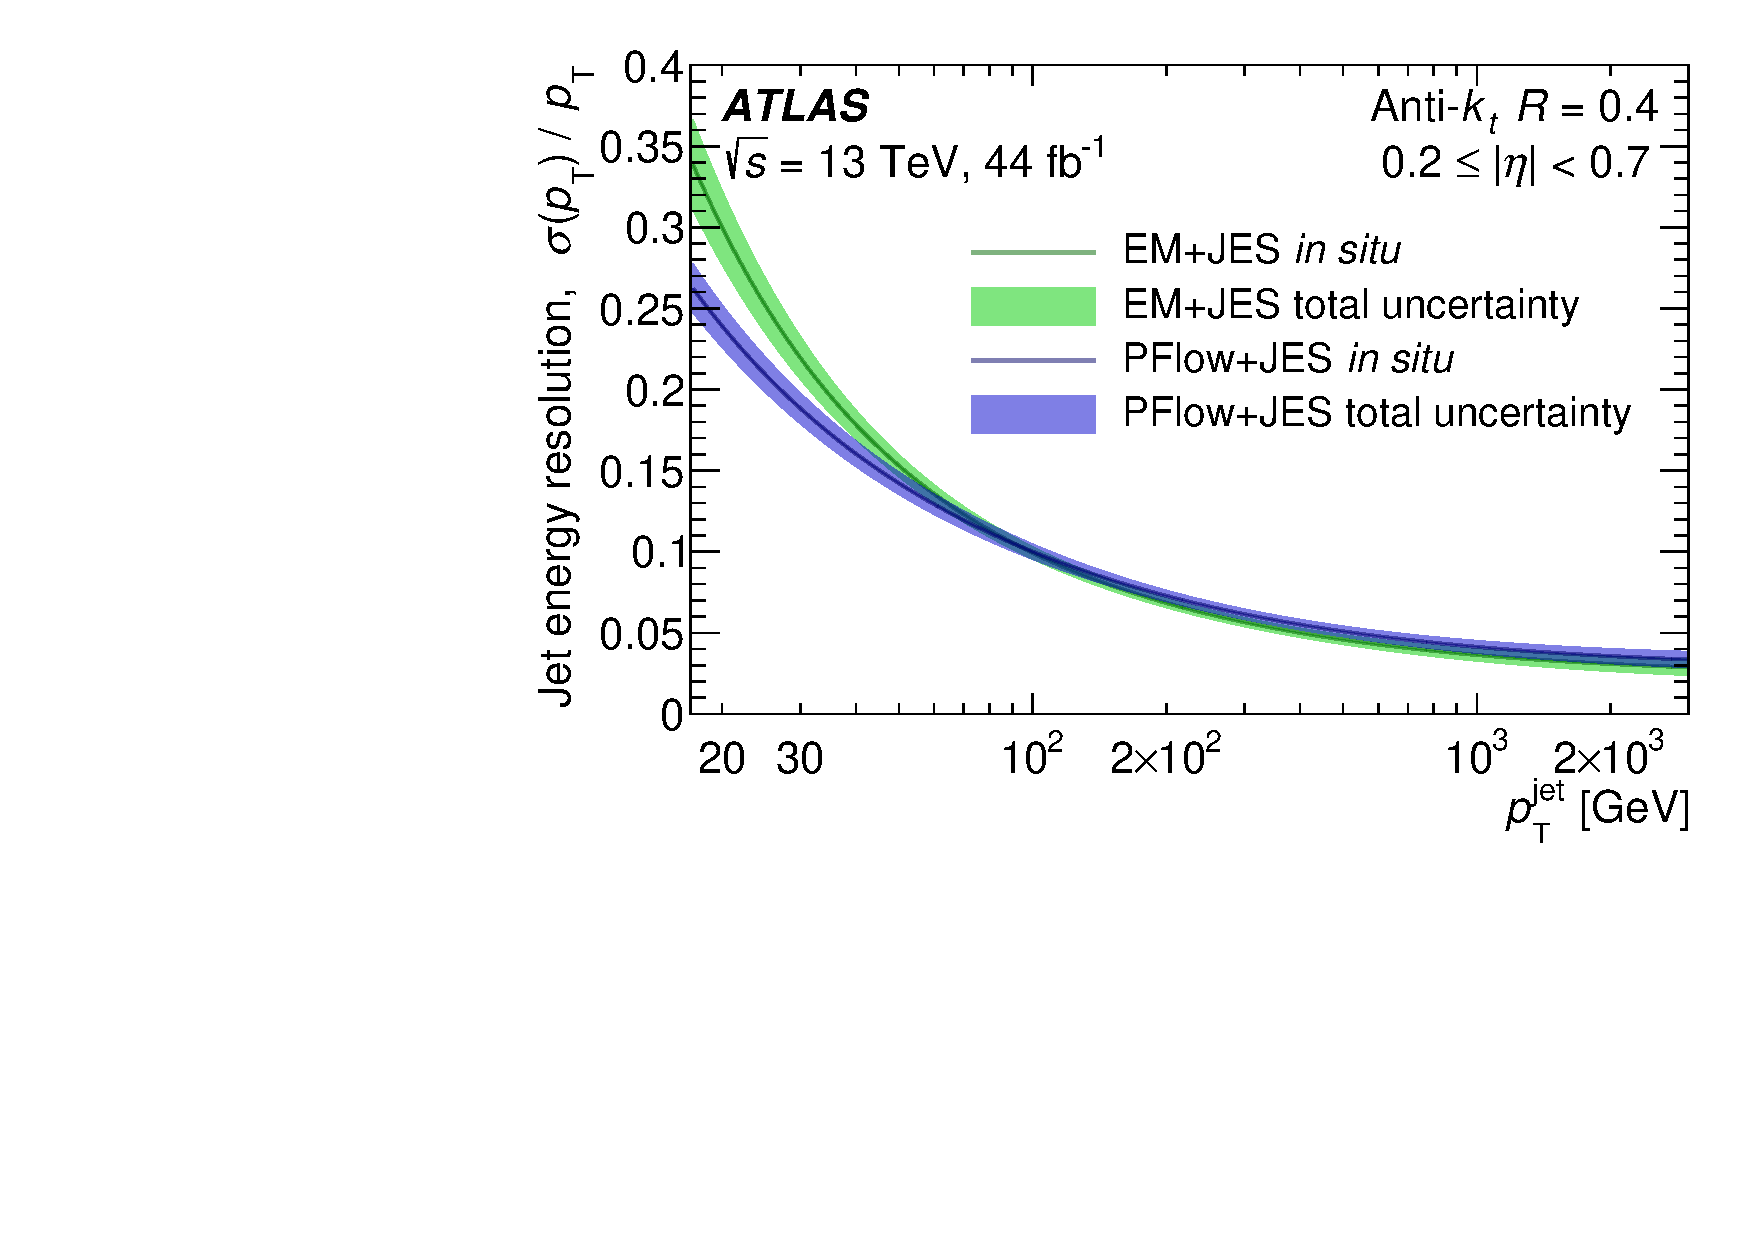
\includegraphics[height=5.4cm]{{figures/cp-graphics/jets/fig_30a}}
	\label{fig:jet-pflow-pt-res}
	}
\subfloat[$\phi$ resolution]{
	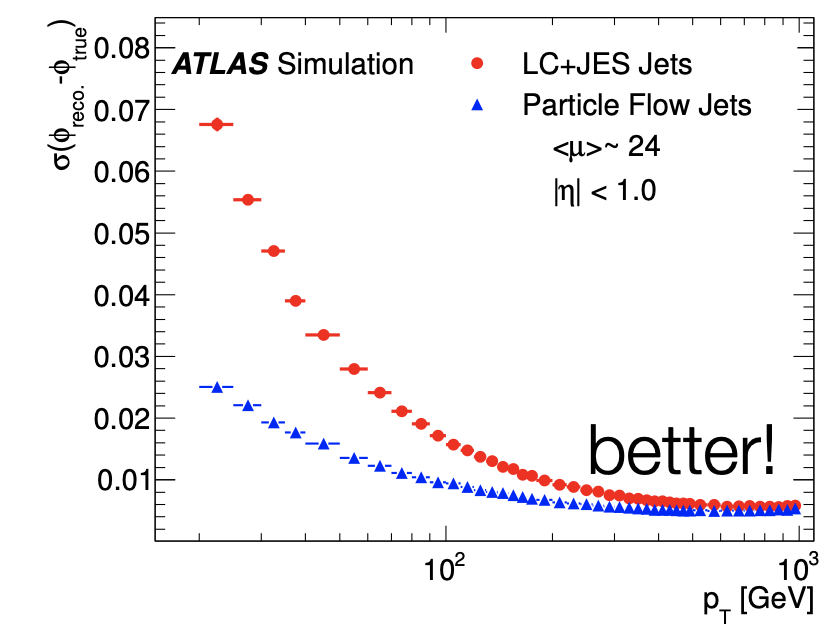
\includegraphics[height=5.4cm]{{figures/cp-graphics/jets/phi_reco}}
	\label{fig:jet-pflow-phi-res}
	}
\caption{Improvement for moving to the PFlow algorithm for jet reconstruction.}
\end{figure}

\subsection{Boosted jets}

\subsection{VR track jets}


\section{Muons}
\label{sec:muons}

Def useful for muon in jet + pt reco correction!!
%Also - for describing the DL1rmu tagger .

%\subsection{Pileup suppression}
%\subsection{Event cleaning}
% I'm tempted to talk about these, but since they're not directly related 
% to the core contributions of my thesis work, I'm going to skip it.
% Oh - I should j add what I put in the int note!!

